\phantomsection
\chapter{Face detection}

\noindent Face detection is the first step after image acquisition. It represents a requirement for a Facial Expression Recognition system. All the background is not taken into account. It allows to focus only on what is interesting in the input image: the face, which helps reducing the processing during the next step that is feature extraction.
\newline

\phantomsection
\section{Detection}

\vspace{\baselineskip}
\noindent Finding out whether or not the input image or video sequence represents or contains a particular object is what is called Detection. Usually after the detection step comes the recognition step. For this system, the recognition step consists in facial expression recognition. But depending on the recognition, there can be another step that is the tracking step. Tracking consists in following a moving target on the images of a video sequence \cite{DIN08}.
\newline

\noindent At a high level, an object detector is a "black box" which gets an image as its input, and gives an annotated image as its output, saying where the object of interest appears in the input image (if it appears...) and the extension of each detected instance of the object \cite{DIN08}. For example, the output can look like in figure~\ref{output_example_face_detection} \cite{DIN08}.
\newline

\begin{figure}[!h]
\begin{center}
\noindent 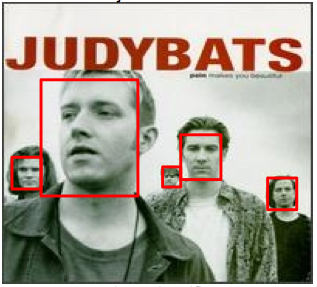
\includegraphics[scale=0.7]{figures/output_example_face_detection} 
\newline
\caption{Example of an output of face detection}
\label{output_example_face_detection}
\end{center} 
\end{figure}

\noindent But at a low level, the basic component of an object detector is just something required to say if a certain sub-region of the original image contains an instance of the object of interest or not. That is what a binary classifier does \cite{DIN08}. For example, what a binary classifier does can look like in figure~\ref{output_example_face_detection_binary_classifier} \cite{DIN08}.
\newline

\begin{figure}[!h]
\begin{center}
\noindent 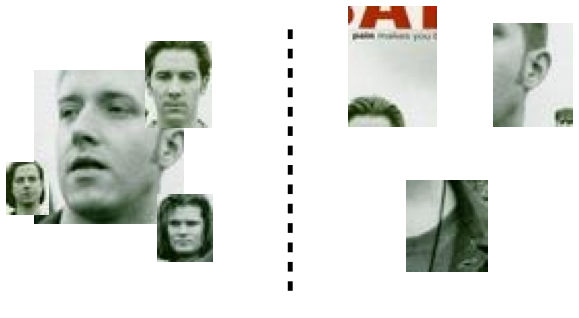
\includegraphics[scale=0.5]{figures/output_example_face_detection_binary_classifier} 
\newline
\caption{Example of what does a binary classifier for face detection}
\label{output_example_face_detection_binary_classifier}
\end{center} 
\end{figure}

\phantomsection
\section{Classifiers}

\vspace{\baselineskip}
\noindent Classification aim to solve the problem of identifying in a set of categories or sub-populations to which a new observation belongs. It is based on a training set of data that contains instances whose category membership is known. An algorithm that implements classification is known as a classifier. Classifiers groups data into categories based on some measure of inherent similarity; for example, the distance between instances, considered as vectors in a multidimensional vector space \cite{CLASS}.
\newline









